\documentclass[aspectratio=169,12pt]{beamer}

%% ── Encodage ─────────────────────────────────────────────────────────────────
\usepackage[utf8]{inputenc}
\usepackage[T1]{fontenc}
\usepackage[provide=*,french,shorthands=off]{babel}
\usepackage{lmodern}

%% ── Design épuré : on part de zéro ──────────────────────────────────────────
\usetheme{default}
\usecolortheme{default}
\setbeamertemplate{navigation symbols}{}
\setbeamertemplate{itemize items}{\textbullet}
\setbeamertemplate{enumerate items}{\insertenumlabel.}

%% ── Couleurs ──────────────────────────────────────────────────────────────────
\definecolor{ink}{RGB}{22, 34, 54}         % presque noir bleu
\definecolor{primary}{RGB}{30, 90, 170}    % bleu principal
\definecolor{accent}{RGB}{255, 140, 0}     % orange accent
\definecolor{lightgray}{RGB}{248, 249, 250}
\definecolor{midgray}{RGB}{108, 117, 125}
\definecolor{success}{RGB}{40, 167, 80}
\definecolor{danger}{RGB}{200, 40, 40}

\setbeamercolor{background canvas}{bg=white}
\setbeamercolor{normal text}{fg=ink}
\setbeamercolor{frametitle}{fg=ink, bg=white}
\setbeamercolor{itemize item}{fg=primary}
\setbeamercolor{enumerate item}{fg=primary}
\setbeamercolor{alerted text}{fg=accent}
\setbeamercolor{example text}{fg=success}
\setbeamercolor{footline}{fg=midgray}

%% ── Fonts ─────────────────────────────────────────────────────────────────────
\setbeamerfont{frametitle}{size=\large, series=\bfseries}
\setbeamerfont{title}{size=\Huge, series=\bfseries}
\setbeamerfont{subtitle}{size=\normalsize, series=\mdseries}
\setbeamerfont{framesubtitle}{size=\small, series=\mdseries}

%% ── Template titre de slide ───────────────────────────────────────────────────
\setbeamertemplate{frametitle}{
  \vspace{0.5em}
  \insertframetitle
  \vspace{-0.2em}
  \par{\color{primary}\rule{0.12\textwidth}{1.5pt}}
  \vspace{0.2em}
}

%% ── Footline simple ───────────────────────────────────────────────────────────
\setbeamertemplate{footline}{
  \leavevmode
  \hbox{
    \begin{beamercolorbox}[wd=.5\paperwidth, ht=2.2ex, dp=1ex, leftskip=0.5em]{footline}
      \tiny\color{midgray} ABIS --- AI Blockchain Immune System
    \end{beamercolorbox}
    \begin{beamercolorbox}[wd=.5\paperwidth, ht=2.2ex, dp=1ex, rightskip=0.5em, right]{footline}
      \tiny\color{midgray}\insertframenumber
    \end{beamercolorbox}
  }
}

%% ── Packages ─────────────────────────────────────────────────────────────────
\usepackage{booktabs}
\usepackage{tabularx}
\usepackage{graphicx}
\usepackage{tikz}
\usetikzlibrary{shapes.geometric, arrows.meta, positioning, backgrounds, calc}
\usepackage{xcolor}
\usepackage{pifont}
\usepackage{array}
\usepackage{listings}
\newenvironment{tightitemize}{%
  \setlength{\topsep}{1pt}\setlength{\partopsep}{0pt}%
  \begin{itemize}\setlength{\itemsep}{1pt}\setlength{\parskip}{0pt}}{\end{itemize}}

\newcommand{\yes}{\textcolor{success}{\ding{51}}}
\newcommand{\no}{\textcolor{danger}{\ding{55}}}
\newcommand{\maybe}{\textcolor{accent}{\textbf{\texttildelow}}}

%% ── Commandes utiles ─────────────────────────────────────────────────────────
\newcommand{\highlight}[1]{\textcolor{primary}{\textbf{#1}}}
\newcommand{\warn}[1]{\textcolor{accent}{\textbf{#1}}}
\newcommand{\good}[1]{\textcolor{success}{\textbf{#1}}}
\newcommand{\bad}[1]{\textcolor{danger}{\textbf{#1}}}

\newcommand{\bigstat}[2]{%
  \begin{center}
    {\fontsize{52}{56}\selectfont\bfseries\color{primary} #1}\\[0.1cm]
    {\normalsize\color{midgray} #2}
  \end{center}
}

%% ── Méta ─────────────────────────────────────────────────────────────────────
\title{ABIS}
\subtitle{AI Blockchain Immune System}
\author{}
\date{}

%% ═════════════════════════════════════════════════════════════════════════════
\begin{document}

%% ── SLIDE 1 : Couverture ─────────────────────────────────────────────────────
{
\setbeamertemplate{footline}{}
\setbeamertemplate{frametitle}{}
\begin{frame}[plain]
  \begin{tikzpicture}[remember picture, overlay]
    % Bande gauche colorée
    \fill[primary] (current page.north west) rectangle
      ([xshift=0.35\paperwidth] current page.south west);
    % Filet accent
    \fill[accent] ([xshift=0.35\paperwidth] current page.north west) rectangle
      ([xshift=0.38\paperwidth] current page.south west);
  \end{tikzpicture}

  \begin{columns}[T]
    \begin{column}{0.35\textwidth}
      \vspace{1.5cm}
      \begin{center}
        
\includegraphics[width=2.5cm]{tek_up_logo.png}\\[0.8cm]
        {\color{white}\large\bfseries ABIS}\\[0.1cm]
        {\color{white!70}\tiny AI Blockchain\\Immune System}
      \end{center}
    \end{column}
    \begin{column}{0.05\textwidth}\end{column}
    \begin{column}{0.57\textwidth}
      \vspace{1.8cm}
      {\color{ink!40}\small Projet de fin d'études --- Tek-UP --- 2025/2026}\\[0.5cm]
      {\color{ink}\Huge\bfseries ABIS}\\[0.1cm]
      {\color{primary}\large\bfseries AI Blockchain Immune System}\\[0.5cm]
      {\color{ink!70}\normalsize
        Détecter et bloquer les attaques\\
        dans les protocoles DeFi\\
        par intelligence artificielle}\\[0.8cm]
      {\color{ink}\small
        \textbf{Yassine Allani} \quad
        \textbf{Maryem El Bekri} \quad
        \textbf{Abderrahmen Ben Khlifa}}
    \end{column}
  \end{columns}
\end{frame}
}

%% ── SLIDE 2 : Le problème en un chiffre ─────────────────────────────────────
{
\setbeamertemplate{footline}{}
\setbeamertemplate{frametitle}{}
\begin{frame}[plain]
  \begin{tikzpicture}[remember picture, overlay]
    \fill[lightgray] (current page.north west) rectangle (current page.south east);
  \end{tikzpicture}
  \begin{center}
    \vspace{0.8cm}
    {\color{midgray}\normalsize La DeFi en 2023}\\[0.4cm]
    {\fontsize{80}{85}\selectfont\bfseries\color{danger} \$1.7B}\\[0.1cm]
    {\color{ink}\Large volés en une seule année}\\[0.6cm]
    {\color{midgray} répartis sur \textbf{400+} incidents majeurs}\\[0.8cm]
    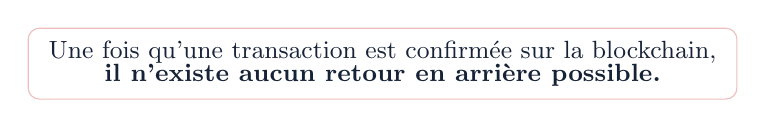
\begin{tikzpicture}
      \node[fill=white, rounded corners=4pt, draw=danger!30,
            minimum width=9cm, minimum height=0.9cm,
            align=center, font=\small\color{ink}]
        {Une fois qu'une transaction est confirmée sur la blockchain,\\[-0.1cm]
         \textbf{il n'existe aucun retour en arrière possible.}};
    \end{tikzpicture}
  \end{center}
\end{frame}
}

%% ── SLIDE 3 : Ce qui rend ça difficile ──────────────────────────────────────
\begin{frame}{Pourquoi c'est difficile à protéger}
  \vspace{0.3cm}
  \begin{columns}[T]
    \begin{column}{0.22\textwidth}
      \begin{center}
        {\color{primary}\fontsize{30}{32}\selectfont\bfseries 12s}\\
        {\tiny\color{midgray} durée d'un bloc\\Ethereum}
      \end{center}
      \vspace{0.3cm}
      {\small Une attaque flash loan s'exécute en \textbf{une seule transaction}. L'agent doit réagir avant le bloc suivant.}
    \end{column}
    \begin{column}{0.02\textwidth}
      {\color{lightgray}\rule{0.5pt}{4cm}}
    \end{column}
    \begin{column}{0.22\textwidth}
      \begin{center}
        {\color{accent}\fontsize{30}{32}\selectfont\bfseries $\infty$}\\
        {\tiny\color{midgray} types d'attaques\\possibles}
      \end{center}
      \vspace{0.3cm}
      {\small Les règles statiques ne couvrent que ce qu'on a \textbf{déjà vu}. Les nouvelles variantes passent à travers.}
    \end{column}
    \begin{column}{0.02\textwidth}
      {\color{lightgray}\rule{0.5pt}{4cm}}
    \end{column}
    \begin{column}{0.22\textwidth}
      \begin{center}
        {\color{primary}\fontsize{30}{32}\selectfont\bfseries N}\\
        {\tiny\color{midgray} wallets\\coordonnés}
      \end{center}
      \vspace{0.3cm}
      {\small Une attaque Sybil utilise plusieurs wallets. Surveiller \textbf{un seul} wallet ne suffit pas.}
    \end{column}
    \begin{column}{0.02\textwidth}
      {\color{lightgray}\rule{0.5pt}{4cm}}
    \end{column}
    \begin{column}{0.22\textwidth}
      \begin{center}
        {\color{accent}\fontsize{30}{32}\selectfont\bfseries ?h}\\
        {\tiny\color{midgray} attaques\\progressives}
      \end{center}
      \vspace{0.3cm}
      {\small Certaines attaques durent des heures, avec de petites transactions qui \textbf{semblent normales} individuellement.}
    \end{column}
  \end{columns}
\end{frame}

%% ── SLIDE 4 : Comparatif solutions ──────────────────────────────────────────
\begin{frame}{Ce qui existe --- et ce qu'il manque}
  \vspace{0.3cm}
  \begin{center}
  \begin{tabular}{lcccc}
    \toprule
    & \small\textbf{Temps réel} & \small\textbf{Réponse auto} & \small\textbf{Comportemental} & \small\textbf{S'adapte} \\
    \midrule
    Audit de code      & \no  & \no  & \no  & \no \\
    Slither / Mythril  & \no  & \no  & \no  & \no \\
    Forta / Tenderly   & \yes & \no  & \maybe & \no \\
    Circuit breaker    & \yes & \yes & \no  & \no \\
    \midrule
    \textbf{ABIS}      & \yes & \yes & \yes & \yes \\
    \bottomrule
  \end{tabular}
  \end{center}
  \vspace{0.5cm}
  \begin{columns}
    \begin{column}{0.48\textwidth}
      {\color{danger}\small $\to$} Les outils existants \textbf{signalent} une anomalie à un humain.\\
      {\color{danger}\small $\to$} L'humain réagit. En attendant, l'argent part.
    \end{column}
    \begin{column}{0.48\textwidth}
      {\color{success}\small $\to$} ABIS agit \textbf{directement sur la blockchain},\\dans le même bloc où l'anomalie est détectée.
    \end{column}
  \end{columns}
\end{frame}

%% ── SLIDE 5 : Notre solution ─────────────────────────────────────────────────
{
\setbeamertemplate{frametitle}{}
\setbeamertemplate{footline}{}
\begin{frame}[plain]
  
\begin{tikzpicture}[remember picture, overlay]
    \fill[ink] (current page.north west) rectangle (current page.south east);
    \fill[primary] ([yshift=-0.08\paperheight]current page.north west) rectangle
      ([yshift=0.08\paperheight]current page.south east);
  \end{tikzpicture}
  \begin{center}
    \vspace{0.5cm}
    {\color{white!50}\small Notre réponse}\\[0.5cm]
    {\color{white}\fontsize{44}{46}\selectfont\bfseries ABIS}\\[0.2cm]
    {\color{white!80}\Large AI Blockchain Immune System}\\[0.8cm]
    {\color{white}\normalsize
    Un agent IA qui surveille chaque transaction,\\
    calcule un score de risque en temps réel,\\
    et \textbf{bloque le wallet directement sur la blockchain}\\
    --- sans attendre qu'un humain lève le doigt.}
  \end{center}
\end{frame}
}

%% ── SLIDE 6 : Architecture ────────────────────────────────────────────────────
\begin{frame}{Vue d'ensemble : 3 couches, un seul objectif}
  \vspace{0.4cm}
  \begin{center}
  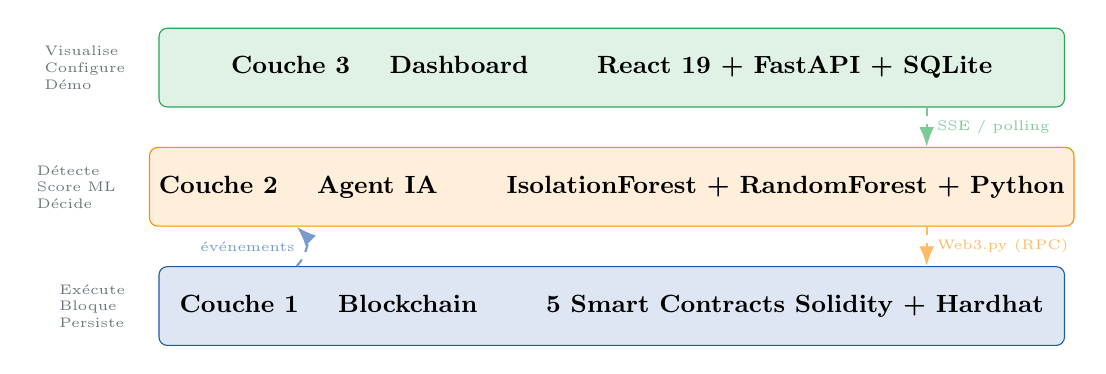
\begin{tikzpicture}[
    layer/.style={rectangle, rounded corners=3pt, minimum width=11.5cm,
      minimum height=1cm, align=center, font=\small\bfseries},
    label/.style={font=\tiny\color{midgray}, align=left},
    arr/.style={-{Latex[length=2.5mm]}, thick}
  ]
    \node[layer, fill=success!15, draw=success] (l3)
      {Couche 3 \quad Dashboard \quad\quad React 19 + FastAPI + SQLite};
    \node[layer, fill=accent!15, draw=accent, below=0.5cm of l3] (l2)
      {Couche 2 \quad Agent IA \quad\quad IsolationForest + RandomForest + Python};
    \node[layer, fill=primary!15, draw=primary, below=0.5cm of l2] (l1)
      {Couche 1 \quad Blockchain \quad\quad 5 Smart Contracts Solidity + Hardhat};

    \node[label, left=0.3cm of l3] {Visualise\\Configure\\Démo};
    \node[label, left=0.3cm of l2] {Détecte\\Score ML\\Décide};
    \node[label, left=0.3cm of l1] {Exécute\\Bloque\\Persiste};

    \draw[arr, success!60, dashed] ([xshift=4cm]l3.south) -- ([xshift=4cm]l2.north)
      node[midway, right, font=\tiny\color{midgray}]{SSE / polling};
    \draw[arr, accent!60, dashed] ([xshift=4cm]l2.south) -- ([xshift=4cm]l1.north)
      node[midway, right, font=\tiny\color{midgray}]{Web3.py (RPC)};
    \draw[arr, primary!60, dashed, bend right=45]
      ([xshift=-4cm]l1.north) to node[left, font=\tiny\color{midgray}]{événements} ([xshift=-4cm]l2.south);
  \end{tikzpicture}
  \end{center}
  \vspace{0.2cm}
  \begin{center}
  {\small\color{midgray}
  Chaque couche est indépendante : si le dashboard tombe, la protection continue.}
  \end{center}
\end{frame}

%% ── SLIDE 7 : Blockchain ─────────────────────────────────────────────────────
\begin{frame}{Couche Blockchain --- le bouclier intégré dans le code}
  \begin{columns}[T]
    \begin{column}{0.50\textwidth}
      Le principe central : le modificateur \texttt{\color{primary}abisGuard}\\[0.15cm]
      {\small Avant d'exécuter quoi que ce soit, le contrat demande à ABIS :
      \textit{«~Ce wallet est-il autorisé~?~»}}\\[0.25cm]
      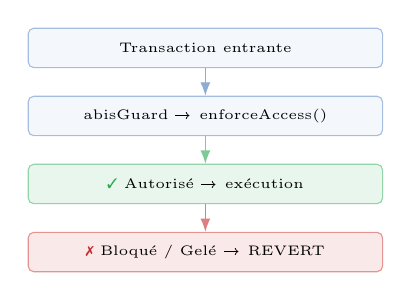
\begin{tikzpicture}[node distance=0.35cm,
        b/.style={rectangle, rounded corners=2pt, draw=primary!40, fill=primary!5,
          minimum width=4.5cm, minimum height=0.5cm, align=center, font=\tiny}]
        \node[b] (tx) {Transaction entrante};
        \node[b, below=of tx] (check) {abisGuard → enforceAccess()};
        \node[b, below=of check, fill=success!10, draw=success!50] (ok) {\yes\ Autorisé → exécution};
        \node[b, below=of ok, fill=danger!10, draw=danger!50] (ko) {\no\ Bloqué / Gelé → REVERT};
        \draw[-{Latex}, primary!50] (tx) -- (check);
        \draw[-{Latex}, success!60] (check) -- (ok);
        \draw[-{Latex}, danger!60] (ok) -- (ko);
      \end{tikzpicture}
    \end{column}
    \begin{column}{0.46\textwidth}
      \textbf{4 niveaux de réponse :}\\[0.25cm]
      \begin{tabular}{p{0.6cm} p{1.8cm} p{2.8cm}}
        {\color{success}\bfseries L1} & WARN & Rate-limit 2min\\[0.15cm]
        {\color{accent}\bfseries L2} & BLOCK & Bloqué 10 min partout\\[0.15cm]
        {\color{accent}\bfseries L2b} & BLOCK\_PROTO & Bloqué sur 1 protocole\\[0.15cm]
        {\color{danger}\bfseries L3} & FREEZE & Gel \textbf{permanent}\\
      \end{tabular}
      \vspace{0.3cm}
      {\small\color{midgray} On sanctionne progressivement selon ce qu'on observe, sans tout bloquer d'un coup.}
    \end{column}
  \end{columns}
\end{frame}

%% ── SLIDE 8 : Agent IA ───────────────────────────────────────────────────────
\begin{frame}{Couche IA --- deux modèles complémentaires}
  \begin{columns}[T]
    \begin{column}{0.48\textwidth}
      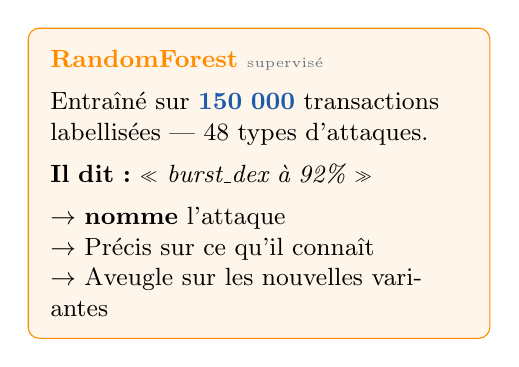
\begin{tikzpicture}
        \node[rectangle, draw=accent, fill=accent!8, rounded corners=4pt,
              minimum width=5.6cm, align=left,
              text width=5.3cm, font=\small, inner sep=8pt] (rf)
          {
            {\color{accent}\bfseries RandomForest} {\color{midgray}\tiny supervisé}\\[0.15cm]
            Entraîné sur \highlight{150 000} transactions\\
            labellisées --- 48 types d'attaques.\\[0.15cm]
            \textbf{Il dit :} \textit{«~burst\_dex à 92\%~»}\\[0.15cm]
            \small$\to$ \textbf{nomme} l'attaque\\
            \small$\to$ Précis sur ce qu'il connaît\\
            \small$\to$ Aveugle sur les nouvelles variantes
          };
      \end{tikzpicture}
    \end{column}
    \begin{column}{0.48\textwidth}
      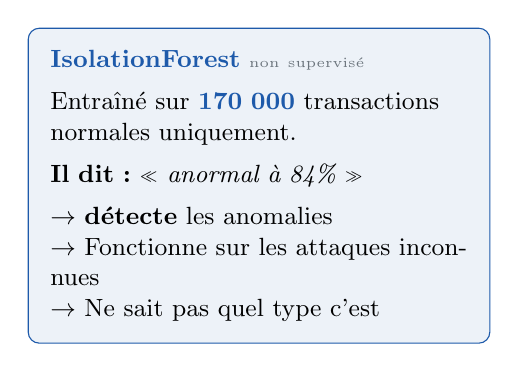
\begin{tikzpicture}
        \node[rectangle, draw=primary, fill=primary!8, rounded corners=4pt,
              minimum width=5.6cm, align=left,
              text width=5.3cm, font=\small, inner sep=8pt] (if)
          {
            {\color{primary}\bfseries IsolationForest} {\color{midgray}\tiny non supervisé}\\[0.15cm]
            Entraîné sur \highlight{170 000} transactions\\
            normales uniquement.\\[0.15cm]
            \textbf{Il dit :} \textit{«~anormal à 84\%~»}\\[0.15cm]
            \small$\to$ \textbf{détecte} les anomalies\\
            \small$\to$ Fonctionne sur les attaques inconnues\\
            \small$\to$ Ne sait pas quel type c'est
          };
      \end{tikzpicture}
    \end{column}
  \end{columns}
  \vspace{0.2cm}
  \begin{center}
    {\small\color{midgray} On combine les deux via un \textbf{scoring hybride} pour avoir le meilleur des deux mondes.}
  \end{center}
\end{frame}

%% ── SLIDE 9 : Scoring hybride ────────────────────────────────────────────────
\begin{frame}{Le scoring hybride --- comment on choisit qui décide}
  \begin{center}
  \scalebox{0.84}{%
  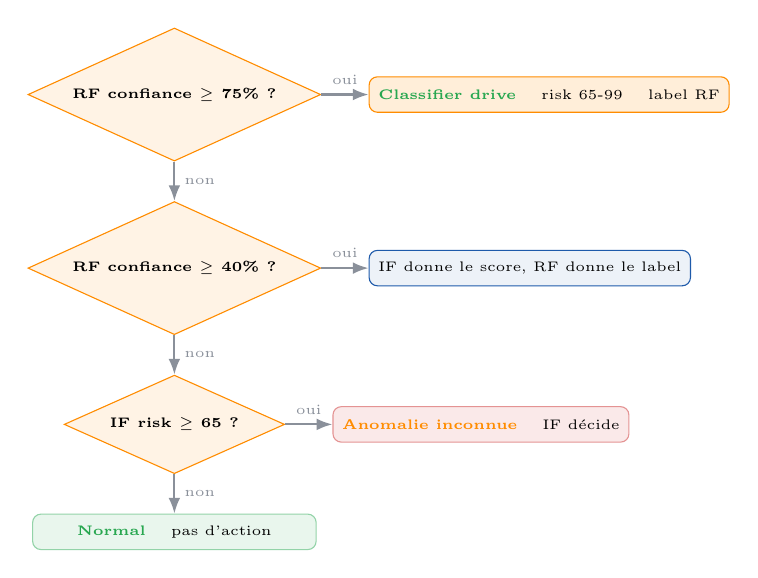
\begin{tikzpicture}[node distance=0.4cm,
    dec/.style={diamond, draw=accent, fill=accent!10, align=center,
      font=\tiny\bfseries, aspect=2.2, minimum width=2.8cm, minimum height=0.5cm},
    res/.style={rectangle, draw=primary, fill=primary!8, rounded corners=3pt,
      align=center, font=\tiny, minimum width=3.6cm, minimum height=0.45cm},
    arr/.style={-{Latex[length=2mm]}, thick, color=ink!50}
  ]
    \node[dec] (c1) {RF confiance $\geq$ 75\% ?};
    \node[res, right=0.6cm of c1, fill=accent!15, draw=accent] (r1)
      {\good{Classifier drive} \quad risk 65-99 \quad label RF};
    \node[dec, below=0.5cm of c1] (c2) {RF confiance $\geq$ 40\% ?};
    \node[res, right=0.6cm of c2] (r2)
      {IF donne le score, RF donne le label};
    \node[dec, below=0.5cm of c2] (c3) {IF risk $\geq$ 65 ?};
    \node[res, right=0.6cm of c3, fill=danger!10, draw=danger!50] (r3)
      {\warn{Anomalie inconnue} \quad IF décide};
    \node[res, below=0.5cm of c3, fill=success!10, draw=success!50] (r4)
      {\good{Normal} \quad pas d'action};

    \draw[arr] (c1) -- node[above, font=\tiny]{oui} (r1);
    \draw[arr] (c1) -- node[right, font=\tiny]{non} (c2);
    \draw[arr] (c2) -- node[above, font=\tiny]{oui} (r2);
    \draw[arr] (c2) -- node[right, font=\tiny]{non} (c3);
    \draw[arr] (c3) -- node[above, font=\tiny]{oui} (r3);
    \draw[arr] (c3) -- node[right, font=\tiny]{non} (r4);
  \end{tikzpicture}}
  \end{center}
  \vspace{-0.2cm}
  \begin{center}
  {\small \textbf{15\%} des détections viennent uniquement de l'IsolationForest --- des attaques que le RF n'avait jamais vues.}
  \end{center}
\end{frame}

%% ── SLIDE 10 : Ce qu'on analyse ──────────────────────────────────────────────
\begin{frame}{Ce qu'on analyse sur chaque transaction}
  \begin{columns}[T]
    \begin{column}{0.52\textwidth}
      \textbf{9 features extraites par fenêtre :}\\[0.02cm]
      {\scriptsize
      \begin{tabular}{ll}
        \toprule
        \textbf{Feature} & \textbf{Ce qu'on mesure} \\
        \midrule
        tx\_count & Nb de tx dans la fenêtre \\
        avg\_value & Montant moyen en ETH \\
        std\_value & Variabilité des montants \\
        dt\_prev & Temps depuis la tx précédente \\
        unique\_to & Nb de destinataires différents \\
        same\_to\_burst & Répétitions vers même cible \\
        value\_eth & Montant de cette tx \\
        contract\_target & Protocole ciblé \\
        window\_s & Fenêtre (5/10/30s) \\
        \bottomrule
      \end{tabular}}
    \end{column}
    \begin{column}{0.44\textwidth}
      \textbf{3 fenêtres courtes :}
      \begin{tightitemize}
        \item \textbf{5 s} --- burst ultra-rapide
        \item \textbf{10 s} --- burst standard
        \item \textbf{30 s} --- comportement général
      \end{tightitemize}
      Score = \textbf{max} des 3 fenêtres.

      \textbf{2 fenêtres longues :}
      \begin{tightitemize}
        \item \textbf{5 min} --- attaques progressives
        \item \textbf{1 h} --- accumulation discrète
      \end{tightitemize}
      \vspace{0.1cm}
      {\small\color{midgray} Les longues fenêtres détectent les attaques furtives passant sous les radars des courtes.}
    \end{column}
  \end{columns}
\end{frame}

%% ── SLIDE 11 : Sybil + lentes ────────────────────────────────────────────────
\begin{frame}{Deux problèmes qu'on a dû résoudre séparément}
  \begin{columns}[T]
    \begin{column}{0.46\textwidth}
      \textbf{\color{primary} Attaques Sybil}\\[0.15cm]
      3 wallets différents font la même attaque au même moment. Pris individuellement, aucun ne dépasse le seuil.\\[0.2cm]
      \textbf{Notre solution :} on regroupe par ``bucket'' de 30s. Si $\geq 3$ wallets attaquent le même protocole $\to$ boost de risque sur les 3.\\[0.2cm]
      {\small\color{midgray} Résultat : \texttt{coordinated\_wallets} et \texttt{sybil\_attack} sont détectées à coup sûr.}
    \end{column}
    \begin{column}{0.04\textwidth}
      {\color{lightgray}\rule{0.5pt}{4cm}}
    \end{column}
    \begin{column}{0.46\textwidth}
      \textbf{\color{accent} Attaques Low \& Slow}\\[0.15cm]
      10 petites transactions à 0.001 ETH, espacées de 2 minutes. Chaque tx est normale vue de près.\\[0.2cm]
      \textbf{Notre solution :} sur les 5min et 1h, on détecte :
      \begin{tightitemize}
        \item Trop de microtransactions $\to$ +25 risque
        \item Montants qui doublent progressivement $\to$ +15 risque
      \end{tightitemize}
      \vspace{0.15cm}
      {\small\color{midgray} Sans ça, \texttt{gradual\_escalation} et \texttt{night\_owl} passaient sous les radars.}
    \end{column}
  \end{columns}
\end{frame}

%% ── SLIDE 12 : Dashboard ─────────────────────────────────────────────────────
\begin{frame}{Le dashboard --- tout voir en temps réel}
  \begin{columns}[T]
    \begin{column}{0.50\textwidth}
      \textbf{4 onglets :}\\[0.15cm]
      \begin{tightitemize}
        \item \textbf{Dashboard} --- métriques live, wallets bloqués avec compte à rebours, incidents filtrables
        \item \textbf{Statistiques} --- distribution des attaques, top wallets, sévérité par bucket
        \item \textbf{Démo} --- lancer n'importe laquelle des 49 attaques et voir la réponse en direct
        \item \textbf{Configuration} --- circuit breaker, whitelist, santé système
      \end{tightitemize}
    \end{column}
    \begin{column}{0.46\textwidth}
      \textbf{Quelques détails techniques :}\\[0.15cm]
      \begin{tightitemize}
        \item Mise à jour en temps réel par \textbf{SSE} (pas de polling lourd)
        \item \textbf{Alertes sonores} avec Web Audio API --- fréquence différente selon WARN / BLOCK / FREEZE
        \item \textbf{WalletModal} --- historique complet + graphique du risk score dans le temps
        \item Mode \textbf{sombre / clair} et raccourcis clavier
      \end{tightitemize}
    \end{column}
  \end{columns}
\end{frame}

%% ── SLIDE 13 : Résultats chiffres ────────────────────────────────────────────
{
\setbeamertemplate{frametitle}{}
\setbeamertemplate{footline}{}
\begin{frame}[plain]
  \begin{tikzpicture}[remember picture, overlay]
    \fill[lightgray] (current page.north west) rectangle (current page.south east);
  \end{tikzpicture}
  \vspace{0.5cm}
  \begin{center}
    {\large\bfseries\color{ink} Ce qu'on a mesuré}\\[0.5cm]
    \begin{tabular}{cccc}
      \begin{minipage}{3.4cm}\centering
        {\fontsize{40}{42}\bfseries\color{primary} 93\%}\\
        {\tiny\color{midgray} taux de détection\\sur 48 types d'attaques}
      \end{minipage}
      &
      \begin{minipage}{3.4cm}\centering
        {\fontsize{40}{42}\bfseries\color{success} $<$3s}\\
        {\tiny\color{midgray} temps de réponse\\moyen (BLOCK)}
      \end{minipage}
      &
      \begin{minipage}{3.4cm}\centering
        {\fontsize{40}{42}\bfseries\color{accent} $<$2\%}\\
        {\tiny\color{midgray} faux positifs\\sur trafic normal}
      \end{minipage}
      &
      \begin{minipage}{3.4cm}\centering
        {\fontsize{40}{42}\bfseries\color{primary} 77}\\
        {\tiny\color{midgray} tests automatisés\\sur 3 niveaux}
      \end{minipage}
    \end{tabular}
    \vspace{0.5cm}
    \par{\color{primary!30}\rule{10cm}{0.5pt}}
    \vspace{0.4cm}

    \begin{tabular}{lccc lccc}
      \tiny Burst (7) & \good{7/7} & \quad &
      \tiny Lending (5) & \good{5/5} & \quad &
      \tiny MEV (4) & \good{4/4} \\
      \tiny Spray (5) & \good{5/5} & &
      \tiny Exploits (5) & \good{5/5} & &
      \tiny Prix (5) & \warn{4/5} \\
      \tiny Drainage (5) & \good{5/5} & &
      \tiny Furtif (5) & \warn{4/5} & &
      \tiny Sybil (4) & \warn{3/4} \\
    \end{tabular}
  \end{center}
\end{frame}
}

%% ── SLIDE 14 : Honnêteté ─────────────────────────────────────────────────────
\begin{frame}{Ce qu'on sait qu'on n'a pas fait parfaitement}
  \begin{columns}[T]
    \begin{column}{0.46\textwidth}
      \textbf{Les 3 vraies limitations :}\\[0.1cm]
      \begin{enumerate}
        \item \textbf{Données synthétiques} --- entraînés sur Hardhat, pas mainnet. Un comportement réel peut différer.\\[0.1cm]
        \item \textbf{Flash loans} --- une attaque en une tx est impossible à stopper avant qu'elle se termine.\\[0.1cm]
        \item \textbf{/unblock sans auth} --- en prod, débloquer devrait exiger une signature admin.
      \end{enumerate}
    \end{column}
    \begin{column}{0.46\textwidth}
      \textbf{Ce qu'on ferait en v2 :}\\[0.15cm]
      \begin{tightitemize}
        \item Fine-tuning sur Uniswap / Aave réels (via The Graph)
        \item Analyse du graphe de tx --- clustering de wallets
        \item Modèle LSTM pour les patterns séquentiels longs
        \item Déploiement L2 (Arbitrum / Optimism)
        \item Gouvernance multi-sig pour les gels permanents
      \end{tightitemize}
    \end{column}
  \end{columns}
\end{frame}

%% ── SLIDE 15 : Conclusion ────────────────────────────────────────────────────
\begin{frame}{En résumé}
  \begin{columns}[T]
    \begin{column}{0.60\textwidth}
      {\small
      ABIS est \textbf{un système complet} --- pas juste un détecteur, pas juste un smart contract.\\[0.1cm]
      On a combiné trois domaines qui ne se parlent pas :
      \begin{tightitemize}
        \item La blockchain pour l'\textbf{enforcement} (irréversible et transparent)
        \item Le machine learning pour la \textbf{détection} (adaptable et comportemental)
        \item Un dashboard pour la \textbf{supervision} et la démonstration
      \end{tightitemize}
      \vspace{0.1cm}
      Le résultat : un wallet malveillant est bloqué \textbf{dans les 3 secondes}, directement au niveau EVM, sans intervention humaine.}
    \end{column}
    \begin{column}{0.36\textwidth}
      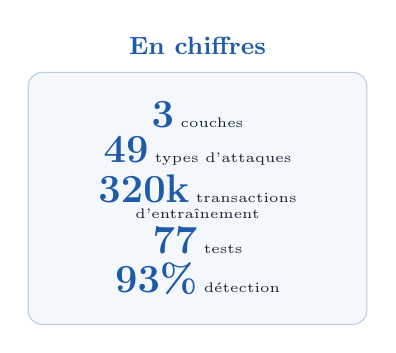
\begin{tikzpicture}
        \node[rectangle, draw=primary!30, fill=primary!5, rounded corners=5pt,
              minimum width=4.3cm, minimum height=3.2cm, align=center] (box) {};
        \node[font=\small\bfseries\color{primary}, above=0.1cm] at (box.north) {En chiffres};
        \node[align=center, font=\tiny\color{ink}] at (box.center) {
          {\color{primary}\bfseries\Large 3} couches\\[0.08cm]
          {\color{primary}\bfseries\Large 49} types d'attaques\\[0.08cm]
          {\color{primary}\bfseries\Large 320k} transactions\\d'entraînement\\[0.08cm]
          {\color{primary}\bfseries\Large 77} tests\\[0.08cm]
          {\color{primary}\bfseries\Large 93\%} détection
        };
      \end{tikzpicture}
    \end{column}
  \end{columns}
\end{frame}

%% ── SLIDE 16 : Questions ─────────────────────────────────────────────────────
{
\setbeamertemplate{footline}{}
\setbeamertemplate{frametitle}{}
\begin{frame}[plain]
  \begin{tikzpicture}[remember picture, overlay]
    \fill[primary] (current page.north west) rectangle
      ([xshift=0.35\paperwidth] current page.south west);
  \end{tikzpicture}
  \begin{columns}[T]
    \begin{column}{0.35\textwidth}
      \vspace{2.5cm}
      \begin{center}
        {\color{white}\Huge\bfseries Merci}\\[0.5cm]
        {\color{white!70}\normalsize Questions ?}
      \end{center}
    \end{column}
    \begin{column}{0.05\textwidth}\end{column}
    \begin{column}{0.57\textwidth}
      \vspace{2.5cm}
      {\color{ink!60}\small Projet réalisé par :}\\[0.4cm]
      {\color{ink}\bfseries Yassine Allani}\\
      {\color{ink}\bfseries Maryem El Bekri}\\
      {\color{ink}\bfseries Abderrahmen Ben Khlifa}\\[0.5cm]
      {\color{midgray}\small Tek-UP --- Université Privée de Tunis\\
      Année académique 2025--2026}\\[0.5cm]
      {\color{primary!60}\small\itshape Démo live disponible sur le dashboard ABIS}
    \end{column}
  \end{columns}
\end{frame}
}

\end{document}
